\documentclass[11pt]{article}
\usepackage[utf8]{inputenc}
\usepackage[T1]{fontenc}
\usepackage{amsmath,amssymb}
\usepackage{booktabs}
\usepackage{graphicx}
\usepackage{geometry}
\geometry{margin=1in}
\usepackage{authblk}
\usepackage[hidelinks]{hyperref}
\usepackage{xurl}
\usepackage{caption}
\usepackage{xcolor}
\usepackage{titlesec}
\usepackage{tikz}
\usepackage[section]{placeins}
\usetikzlibrary{positioning,arrows.meta}
\definecolor{navy}{HTML}{1A3A5C}
\definecolor{accent}{HTML}{2563EB}
\titleformat{\section}{\normalfont\Large\bfseries\color{navy}}{\thesection}{1em}{}
\titleformat{\subsection}{\normalfont\large\bfseries\color{accent}}{\thesubsection}{1em}{}
\graphicspath{{figures/}}
\setlength{\emergencystretch}{2em}

\newcommand{\zindiuser}{\texttt{craigouma}}
\newcommand{\gap}{\operatorname{gap}}

\title{\textbf{Unnamed Local Roads on Tribal Reservations: A Coverage Gap
the Bias Scorecard Cannot See}}

\author[1]{Craig Carlos Ouma\thanks{%
Correspondence: \texttt{craigcarlos95@gmail.com}. Zindi: \zindiuser{} (solo).
Leaderboard submissions tied to the methodology: S24 (\texttt{EC3xBxjr}) and
S19 (\texttt{Ekx9Rx3y}).
Entry for Best Bias Discovery, Bias Bounty Mapping Equity Challenge. The
full methodology is submitted separately for Best Documentation.}}
\affil[1]{Independent Researcher}
\date{\today}

\begin{document}
\maketitle

\begin{abstract}
\noindent
The challenge's coverage measures and every Bias Scorecard metric count road
length and features, so a road drawn without a name counts as fully covered.
Using only the challenge data (Overture Maps release 2026-08-19.0 and the
strata tables), this entry measures the share of drivable road length with no
name in each of 9,794 scored tracts and compares tribal with non-tribal
tracts within the same region and rurality class. On 80 federally recognised
reservation tracts, local streets are unnamed 9.5 percentage points more
often than on matched non-tribal tracts (95\,\% county bootstrap interval 3.5
to 14.7), while highways on the same tracts show no difference ($-0.4$). The
Osage Reservation reaches $+27.6$ points, with 57\,\% of its drivable length
unnamed. In 19 reservation tracts, home to 55,092 people, at least 30\,\% of
local street length has no name, against 13\,\% of comparable non-tribal
tracts. Several of these tracts combine unnamed streets with recent wildfire
and high social vulnerability. Emergency dispatch, evacuation orders and
relief operations locate people by street name, so these residents are the
hardest to reach in exactly the events the challenge regions face.
\end{abstract}


\section{The pattern and why the scorecard cannot see it}

Every coverage measure in this challenge, and every metric on the Bias
Scorecard, counts length or features. A road segment that Overture holds
without a name adds as much length as a named one, so a tract whose roads
are all drawn but half unnamed scores as fully covered. The name is what
emergency services use. A caller gives an address, computer-aided dispatch
validates it against road centrelines that carry street names and address
ranges \cite{nena006}, and routing tools give instructions by street name.
This section shows that on federally recognised reservations a much larger
share of the local street network has no name in Overture than on comparable
non-tribal tracts, while the highways through the same reservations are
named as often as anywhere else.

\section{Measure and comparison}

For each scored tract the measure is the share of drivable road length
(Overture \cite{overture} \texttt{roads} layer, classes motorway to unclassified, clipped to
the tract) whose \texttt{names.primary} is empty. It is computed separately
for the local classes (tertiary, residential, unclassified) and the named
classes (motorway, trunk, primary, secondary). Tracts are tribal when the
challenge's tribal overlap table links them to an American Indian, Alaska
Native or Native Hawaiian area, split into legal areas (reservations and
off-reservation trust land) and statistical areas (Oklahoma Tribal
Statistical Areas, OTSAs).

Rurality changes naming a great deal: in South-Central Texas the unnamed
share is 8\,\% in metropolitan tracts and 29\,\% in rural ones. Tribal tracts
are therefore compared with non-tribal tracts in the same region and RUCA
class \cite{ruca} (metropolitan, micropolitan, small town, rural), and the cell
differences are averaged with weights equal to the number of tribal tracts
in each cell. Intervals come from 1,000 bootstrap resamples of whole
counties, which keeps neighbouring tracts that share mapping history
together. All numbers come from stage 04 run
\texttt{20261029-2348-04\_analysis-503f5c5} on the challenge data only;
county names come from the Census 2020 county code list \cite{countycodes}.

\paragraph{Reproducing the finding.} Road length comes from
\nolinkurl{<region>-overture-roads.parquet} (classes motorway, trunk, primary,
secondary, tertiary, residential, unclassified), as geodesic metres of each
segment clipped to the tract polygons in \nolinkurl{<region>-census-tracts.parquet};
a segment is unnamed when \texttt{names.primary} is null. The tribal kind comes
from \nolinkurl{<region>-strata-tract-table.parquet}: a tract is a reservation
tract when \texttt{tribal\_legal} is true and a statistical-area tract when
\texttt{tribal\_any} is true and \texttt{tribal\_legal} is false; area names come
from \texttt{aiannh\_name} in \nolinkurl{<region>-tribal-tract-table.parquet}. The
rurality class maps \texttt{ruca\_primary} 1 to 3 to metropolitan, 4 to 6 to
micropolitan, 7 to 9 to small town and 10 to rural. Tracts with no drivable
road are left out, and tracts with no local road are left out of the local
comparison. In each region and class cell holding both groups, the mean
tribal share minus the mean non-tribal share is taken, and the cells are
averaged with weights equal to their tribal tract counts. The interval
resamples counties (the first five GEOID digits) with replacement 1,000
times and reports the 2.5th and 97.5th percentiles, dropping resamples in
which no cell holds both groups.

\section{Evidence}

Table~\ref{tab:contrast} and Figure~\ref{fig:contrast} give the matched
differences. On the 80 reservation tracts, local streets are unnamed 9.5
percentage points more often than on matched non-tribal tracts (95\,\%
interval 3.5 to 14.7). The highways on the same tracts show no difference
($-0.4$, interval $-7.3$ to 5.6), so the gap sits on the streets where people
live and the measure is not picking up a regional habit of leaving highways
unnamed. The difference holds in each region with enough reservation tracts
to test: Maricopa (37 tracts, $+7.3$), Eastern Washington (16, $+4.5$) and
Eastern Oklahoma, where the Osage Reservation reaches $+27.6$ (9.8 to 29.6).
Northern California's 13 reservation tracts point the same way with an
interval that includes zero.

\begin{table}[htbp]
\centering
\small
\caption{Tribal minus non-tribal unnamed share of drivable length, matched
within region and RUCA class, in percentage points, with 95\,\% county
bootstrap intervals.}
\label{tab:contrast}
\begin{tabular}{llrrr}
\toprule
Tribal tracts & Roads & Tracts & Difference & Interval \\
\midrule
Reservations, all regions & local & 80 & $+9.5$ & 3.5 to 14.7 \\
Reservations, all regions & all drivable & 80 & $+8.3$ & 2.9 to 13.5 \\
Reservations, all regions & named classes & 79 & $-0.4$ & $-7.3$ to 5.6 \\
Osage Reservation, Eastern Oklahoma & local & 13 & $+27.6$ & 9.8 to 29.6 \\
Reservations, Maricopa & local & 37 & $+7.3$ & 3.0 to 10.9 \\
Reservations, Eastern Washington & local & 16 & $+4.5$ & 0.0 to 14.8 \\
Reservations, Northern California & local & 13 & $+3.8$ & $-2.9$ to 10.1 \\
OTSAs, Eastern Oklahoma & local & 792 & $+3.0$ & $-6.0$ to 7.5 \\
\bottomrule
\end{tabular}
\end{table}

\begin{figure}[htbp]
\centering
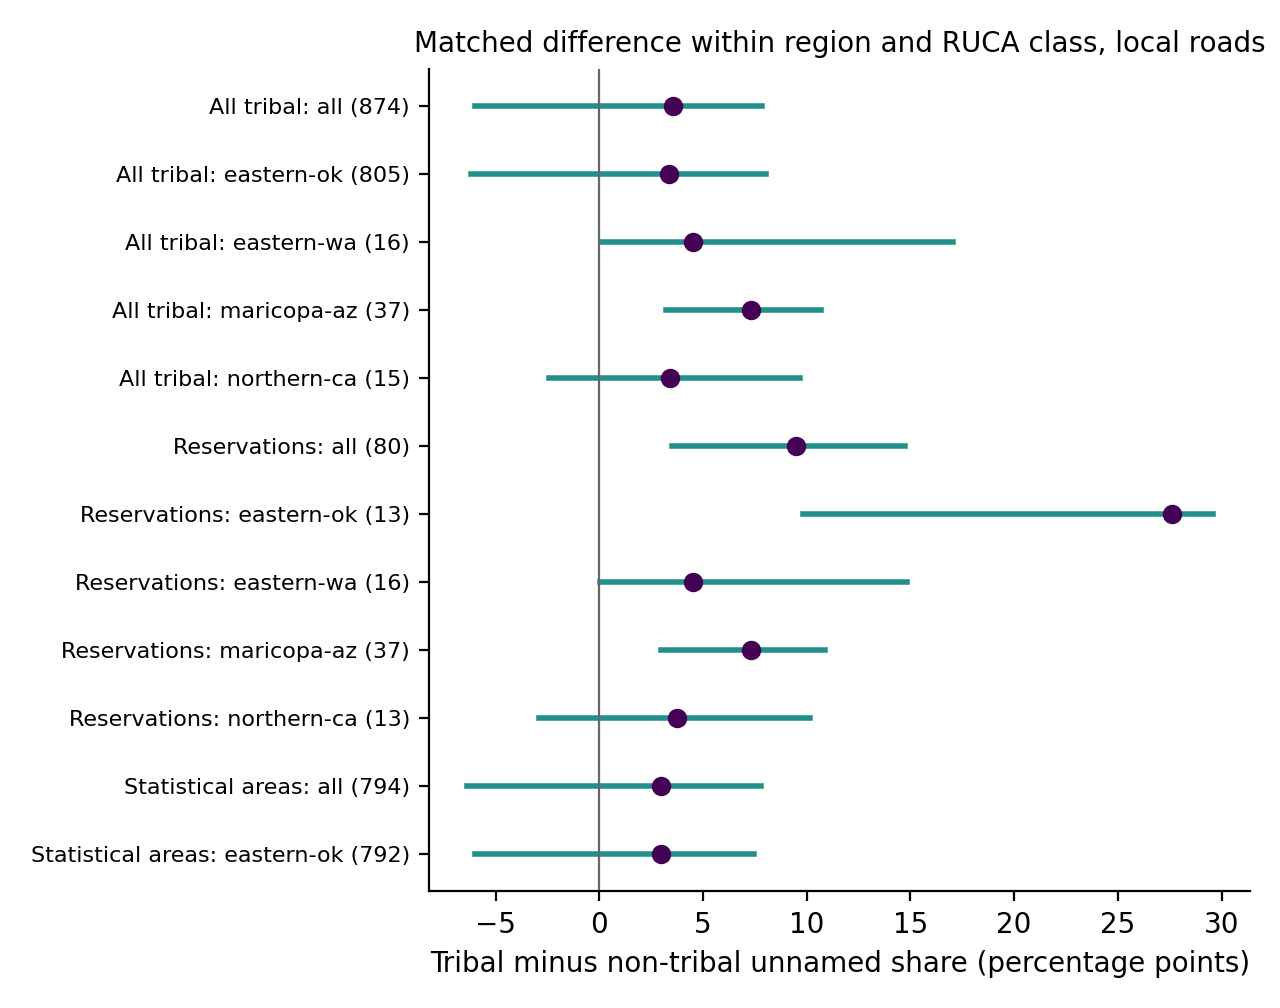
\includegraphics[width=0.68\textwidth]{fig_contrast_local.png}
\caption{Matched difference in the unnamed share of local street length,
tribal minus non-tribal tracts, with 95\,\% county bootstrap intervals.
Numbers in brackets are tribal tracts.}
\label{fig:contrast}
\end{figure}

The OTSAs hold the largest unnamed networks in absolute terms: 13,066\,km of
unnamed drivable road in the Cheyenne and Arapaho OTSA (47\,\% of its
network) and 8,831\,km in the Choctaw OTSA (34\,\%). After matching they do
not separate from non-tribal tracts, because 792 of Eastern Oklahoma's 1,192
scored tracts lie in an OTSA and only 43 non-tribal tracts outside its
metropolitan areas remain to compare with. The OTSA result is therefore
unresolved by this design, and the claim made here is limited to
reservations.

The 80 reservation tracts hold 294,612 residents and 8,266\,km of unnamed
drivable road. In 19 of them, home to 55,092 people, at least 30\,\% of local
street length has no name. That is 24\,\% of reservation tracts, against
13\,\% of non-tribal tracts once those are weighted to the same mix of
rurality.

Table~\ref{tab:tracts} names the reservation tracts with the most unnamed
road, with their wildfire history and social vulnerability from the
challenge's strata tables. Several of them combine a largely unnamed street
network with recent fire and high vulnerability. Tract 9400.04 in Osage
County, Oklahoma has 78\,\% of its drivable length unnamed and 29\,\% of its
land burned between 2015 and 2023. Tract 9400 in Ferry County, Washington,
on the Colville Reservation, has 498\,km of unnamed road, 27\,\% of its land
burned since 2015 and an SVI percentile of 0.84. Tracts 9408 and 9411 in
Pima County, Arizona, on the Tohono O'odham Nation Reservation in the
Sonoran Desert, have SVI percentiles of 0.96 and a third or more of local
street length unnamed.

\begin{table}[htbp]
\centering
\small
\caption{Reservation tracts with the most unnamed drivable road. Local:
unnamed share of local street length. Burned: share of land burned
2015 to 2023 (MTBS). SVI: CDC SVI 2022 overall percentile \cite{svi}.}
\label{tab:tracts}
\resizebox{\textwidth}{!}{%
\begin{tabular}{llllrrrrr}
\toprule
GEOID & Tract & County & Reservation & Unnamed km & All & Local & Burned & SVI \\
\midrule
40113940004 & 9400.04 & Osage, OK & Osage & 606 & 0.78 & 0.86 & 0.29 & 0.48 \\
40113940003 & 9400.03 & Osage, OK & Osage & 524 & 0.62 & 0.62 & 0.12 & 0.74 \\
53019940000 & 9400 & Ferry, WA & Colville & 498 & 0.34 & 0.36 & 0.27 & 0.84 \\
04001970202 & 9702.02 & Apache, AZ & Zuni & 462 & 0.35 & 0.39 & 0.00 & 0.54 \\
40113940011 & 9400.11 & Osage, OK & Osage & 454 & 0.74 & 0.71 & 0.12 & 0.58 \\
06023010102 & 101.02 & Humboldt, CA & Yurok & 387 & 0.32 & 0.32 & 0.20 & 0.61 \\
04001970502 & 9705.02 & Apache, AZ & Fort Apache & 385 & 0.23 & 0.23 & 0.02 & 0.66 \\
04019940800 & 9408 & Pima, AZ & Tohono O'odham & 384 & 0.40 & 0.45 & 0.03 & 0.96 \\
40113940001 & 9400.01 & Osage, OK & Osage & 327 & 0.61 & 0.68 & 0.37 & 0.83 \\
04017940100 & 9401 & Navajo, AZ & Fort Apache & 324 & 0.47 & 0.52 & 0.07 & 0.87 \\
\bottomrule
\end{tabular}}
\end{table}

\section{Consequences}

\paragraph{Emergency dispatch.} An address on a road with no name in the map
cannot be matched to a centreline, so a 911 call from it geocodes to a
nearby named road, a ZIP centroid or nothing. On a reservation, response is
often shared between tribal, county, state and federal agencies, and units
arriving from outside lack the local knowledge that substitutes for a street
name. On the Osage Reservation, where 57\,\% of the drivable length has no
name and single tracts reach 78\,\%, a crew from a neighbouring county
routed by a tool built on open map data receives instructions in which most
turns are onto an unnamed road.

\paragraph{Evacuation routing.} Wildfire evacuation orders name the roads
to leave by and the zones they bound. Where a third of the local network is
unnamed, as on the Colville and Yurok tracts with a fifth to a quarter of
their land burned since 2015, zone maps and routing products drawn from open
data cannot describe the egress routes that residents of those roads would
need.

\paragraph{Disaster relief.} Damage assessment, supply distribution and
welfare checks during extreme heat, which the Tohono O'odham tracts face each
summer, are organised by address. Households on unnamed roads drop out of
address-based lists and have to be found by coordinates.

\paragraph{Why the scorecard misses it.} The Road Network Equity Ratio and
the other scorecard metrics compare lengths and counts, and the transport
component itself compares only motorway to secondary length. A reservation
whose streets are drawn but unnamed has full road coverage by every one of
these measures. The disparity becomes visible only through an attribute,
the name, that none of them reads.

\section{Reproducibility}

Every number comes from stage 04 run
\texttt{20261029-2348-04\_analysis-503f5c5} of the challenge pipeline (seed
20261025, 1,000 county bootstrap resamples per interval), which read only the
challenge bucket \cite{bucket} and the Census 2020 county code list \cite{countycodes}, retrieved 29
October 2026, for county names. A
second run with the same code reproduced every number and figure exactly.
The tract-level tables (\texttt{unnamed\_worst\_reservation\_tracts.csv},
\texttt{unnamed\_by\_tribal\_area.csv}) are produced by the same run.
The measure reads Overture names as published. A road may carry a name in a
local addressing system that Overture does not hold; in that case the open
map lacks the name, which is the gap being measured.

\begin{thebibliography}{99}
\bibitem{bucket}
Humane Intelligence (2026). Bias Bounty Mapping Equity Challenge data
repository and README. Source Cooperative.
\url{https://source.coop/humane-intelligence/bias-bounty-mapping-equity-challenge}

\bibitem{overture}
Overture Maps Foundation (2026). Overture Maps release 2026-08-19.0 and
schema documentation. \url{https://docs.overturemaps.org/}

\bibitem{nena006}
National Emergency Number Association (2022). NENA Standard for NG9-1-1 GIS
Data Model, NENA-STA-006.2-2022.

\bibitem{svi}
Centers for Disease Control and Prevention and ATSDR (2024). CDC/ATSDR Social
Vulnerability Index 2022.

\bibitem{ruca}
USDA Economic Research Service (2025). Rural-Urban Commuting Area codes,
2020.

\bibitem{countycodes}
US Census Bureau. 2020 national county code list
(\texttt{national\_county2020.txt}). Retrieved 29 October 2026.
\url{https://www2.census.gov/geo/docs/reference/codes2020/national_county2020.txt}

\end{thebibliography}

\end{document}
